\part{Plateforme du comportement des occupants}

\chapter{Simulation Stochastique à base d'agents (MASS)}
\label{MASS}

--------------------Changer le titre car c'est maladroit-------------------------
--------------------Comparer Model Exchange avec Co-simulation-------------------

L'État de l'art sur la modélisation du comportement des occupants nous a donc amené à nous orienter vers une modélisation stochastique à base d'agents. Le travail réalisé n'aurait pas été possible sans l'Université de Nottingham et particulièrement son unité de recherche \textit{Building and Urban Physics and Head of the Energy and Sustainability Research Division} qui nous a fait partager son travail sans contrepartie. Avant de rentrer dans le cœur du chapitre nous tenons alors à réitérer nos remerciements à Darren Robinson, Jacob Chapman et l'ensemble de équipe. 

Ce chapitre présente dans un premier temps l'architecture par laquelle se fait l'intégration des modèles du comportement des occupants dans les programmes de simulation énergétique puis présente dans un second temps la stratégie générale de développement de l'outil MASS.

\section{Intégration de modèles comportementaux aux logiciels de simulations thermiques dynamiques}

S'inspirer de la partie 6 du papier: "Occupant behavior modeling for building performance simulation: Current state and future challenges"  Da Yan, 2015. Puis ajouter les intérêts de la co-simulation p140 2012-Gaaloul thèse.



\section{MASS: Un Système Multi-Agents simplifié}

Nous avons proposé une définition systèmes multi-agents dans la section \ref{Systèmes Multi-Agents}. Cette définition est controversée et extrêmement large. Si on se tient à la définition la plus rigoureuse des agents par l'informaticien Ferber \cite{Ferber-95} alors MASS n'est pas un système multi-agents. En effet, selon cette définition un agent est une entité physique ou virtuelle:
\begin{itemize}
  \item qui est capable de percevoir son environnement,
  \item qui est capable d'agir dans son environnement, 
  \item qui peut communiquer directement avec d'autres agents,
  \item qui est influencé par un ensemble de tendances,
  \item qui possède des ressources propres,
  \item qui possède des compétences et offre des services,
  \item et qui peut éventuellement se reproduire, mourir et changer d'état
\end{itemize}
Or les agents de MASS n'ont ni la capacité de communiquer avec d'autres agents, ne sont pas influencés par des tendances, n'ont pas de ressources propres et ne possèdent pas de compétences particulières.

Néanmoins, dans son livre, Ferber \cite{Ferber-95} donne également la définition d'un agent réactif tropique. En opposition à un agent réactif pulsionnel qui est dirigé par des buts, l'agent réactif tropique ne répond qu'à des stimuli de l'environnement, son comportement étant guidé intégralement par l'état local du monde dans lequel il se trouve plongé. Il s'agit alors d'actions totalement réflexes sans but ni état interne. On peut alors en toute légitimité appeler les agents de MASS des agents réactifs tropiques, et son ensemble un système multi-agents réactif tropique.

\section{Architecture du modèle}

Due à leurs nature intrinsèquement différente, le comportement des occupants et celui des bâtiments sont modélisés deux différents paradigmes. Le comportement des occupants est décrit par MASS qui est une modélisation à base d'agents, alors la modélisation des bâtiments est décrit par des équations différentielles typiques des modélisations thermiques dynamiques. Une telle différence de ces systèmes complexes ne peut pas être modélisée efficacement dans un outil unique, le couplage par FMI est alors une solution. [Coupling OB with a building energy model - A FMI application, Plessis, 2014]

Interet de la dll: L'utilisation d'une bibliothèque (dll) est un excellent moyen de réutiliser le code. Au lieu d'implémenter les mêmes routines dans chaque programme que vous créez, vous les écrivez une seule fois, puis vous les référencez dans les applications qui requièrent ces fonctionnalités. En plaçant du code dans la DLL, vous économisez de l'espace dans chaque application qui la référence, et vous pouvez mettre à jour la DLL sans recompiler toutes les applications.

Ce paragraphe présente comment le FMU (Functional Mockup Unit) est implémenté pour la co-simuilation avec Energyplus. L'utilisation d'une interface externe via FMU à EnergyPlus a été réalisé pour la première fois en 2013 par le Lawrence Berkeley National Laboratory de Berkeley et présenté par Nouidui et al. \cite{Nouidui-13}. Ils ont présenté les concepts des FMI et FMU ainsi que proposé des cas d'applications sur un système CVC et sur le contrôle des stores.

....Continuer en se basant sur l'article de Nouidui \cite{Nouidui-13}.... et sur l'Annex 60

Le développement de la plateforme multi-agents est réalisé en C++, comme le montre la figure \ref{fig:CPP}, ce langage est de bas niveau, c'est à dire proche de l'assembleur de l'ordinateur. Son approche est délicate car le développeur nécessite de bien comprendre le fonctionnement de base de l'ordinateur et notamment la gestion dynamique de la mémoire. En revanche, il est très répandu donc bien documenté, il est rapide donc bien adapté pour de la co-simulation avec un logiciel externe, il est portable donc un même source code peut être transformé en exécutable Windows, MAC OS et Linux et il est surtout multi-paradigme donc son code est organisé en blocs réutilisables grâce à la programmation orientée objet (POO).

\begin{figure}[H]
\centering
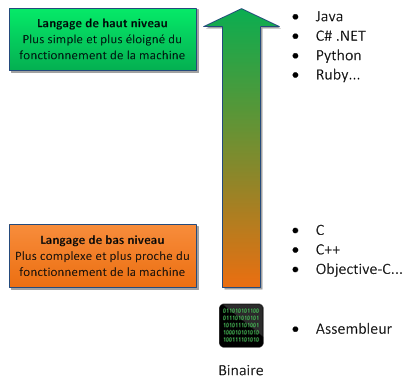
\includegraphics[scale=0.8]{Images/CPP}
\caption{Différents niveaux de langage}
\label{fig:CPP}
\end{figure}

L'idée générale du développement est de pouvoir greffer aux logiciels existant un module du comportement des occupants qui peut être utilisé de trois manières différentes. Premièrement, le modèle du comportement peut fonctionner indépendamment de l'outil de STD comme un fichier exécutable pour pré-calculer les présences et les activités. Deuxièmement, il peut être intégré au programme de simulation énergétique comme une bibliothèque dynamique, appelée en anglais \textit{Dynamic Link Library} (DLL). Troisièmement, le modèle du comportement peut-être utilisé via une co-simulation avec d'autres programmes.

D'un point de vue technique la co-simulation dynamique de MASS et d'EnergyPlus est réalisée grâce à l'outil FMI (\textit{Function Mock-up Interface)} qui utilise dans notre cas la combinaison de fichiers XML et de programmes C++. En réalité l'outil FMI nécessite un composant qui va l'implémenter, c'est le FMU (\textit{(Function Mock-up Unit)}. EnergyPlus est le co-simulateur dynamique maître car il contrôle l'échange de données et la synchronisation des programmes C++ qui composent le FMU.

Pour utiliser le FMU en co-simulation, il y a deux étapes importantes: le pré-processus et la co-simulation. L'étape de pré-processus génère une section du fichier d'entrée d'EnergyPlus (*.idf) qui peut être utilisée pour configurer le FMU pour la co-simulation. Ce fichier d'entrée définit les entrées et les sorties pour d'une part EnergyPlus mais également pour le FMU. Deuxièmement, l'étape de co-simulation exécute la simulation elle-même avec les échanges dynamiques entre EnergyPlus et le FMU.

La figure \ref{fig:FMU} montre les étapes du pré-processus pour la co-simulation via FMU.

\begin{figure}[H]
\centering
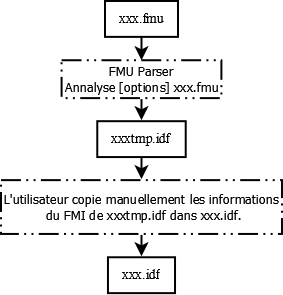
\includegraphics[scale=0.4]{Images/FMU_Pre-process}
\caption{Cheminement du pre-processus du FMU}
\label{fig:FMU}
\end{figure}

The FMI development is part of the ITEA2 MODELISAR project(2008 - 2011; 29 partners, Budget: 30 Mill. \euro). FMI development initiated, organized and headed by Daimler AG (Mercedes-Benz)

Dans MASS un agent correspond à une personne individuel et une famille correspond à un groupe d'agents.

\section{Interopérabilité des outils de MASS}

Intérêt de la co-simulation: p140 2012-Gaaloul thèse.

Comment utiliser MASS pour une co-simulation avec TRNSYS, COMFIE, ...? 2012-Gaaloul-Interopérabilité basée sur les standards Modelica et composant logiciel pour la simulation énergétique des systèmes de bâtiment

\section{Fonctionnement du FMI}

Le FMI standard compose le cœur de la co-simulation, il permet de faire l'interface entre le logiciel de simulation dynamique et la plateforme MASS. La Figure \ref{fig:diagramOfTheCo-Simulation} détail le processus et le fonctionnement.

\begin{figure}[H]
\centering
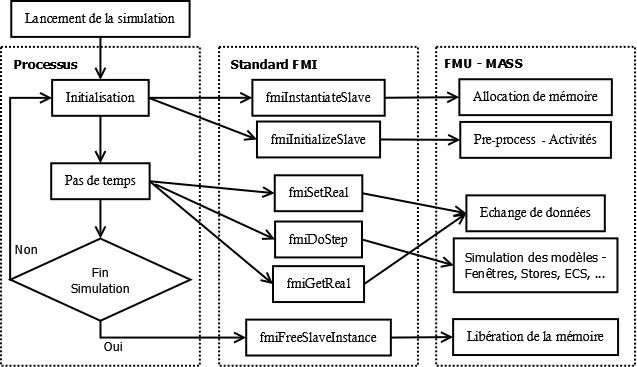
\includegraphics[scale=0.45]{Images/diagramOfTheCo-Simulation}
\caption{Diagramme de l'utilisation de l'interface de co-simulation FMI}
\label{fig:diagramOfTheCo-Simulation}
\end{figure}

\section{Stratégie générale de développement}



\section{Validation des modèles du comportement des occupants}

Le développement de modèles résulte de campagne de mesures et d'analyses. Or, une étape fondamentale est parfois négligée, il s'agit de celle de validation des modèles. La majorité des processus de validations passés sont limités à la comparaison des sorties de la simulation aux données dans le même contexte que le modèle a été développé. Cela mène à une surestimation des performances du modèle. Cette section présente les approches de validation de modèles pour le comportement des occupants.
On recense deux types de validation; les procédures de validation internes et les procédures de validation externe. Steyerberg \cite{Steyerberg-03} définit les données externes comme des données venant de mesures différentes mais venant tout de même d'une population plausiblement liée.
Dans le contexte du comportement des occupants dans les bâtiments il y a au moins trois dimensions externes à considérer: le temps, l'environnement et les occupants. La question est alors de connaître quelles dimensions doivent varier pour obtenir des données externes. Si l'objectif du modèle est de modéliser un comportement dans un bâtiment particulier alors une variation dans le temps peut être suffisante pour l'obtention de données externes. Or si l'objectif du modèle est d'être généralisé à des occupants et à des bâtiments divers alors davantage de données issus d'autres occupants et d'autres bâtiments est nécessaire.
[Revisiting validation methods of OB models - Wolf - 2015]


A mettre ailleurs: Le traitement de l'ensemble des résultats issus des simulations sont traité grâce au langage R. Le point fort de R par rapport à un logiciel à menus déroulants est dans la possibilité de programmer une suite d'analyses successivement. Comme les autres langages, R possède des structures de contrôle proches des langages Java et C/C++.


% Prévoir à la fin de la thèse une figure qui montre les éléments qui ont été considérés dans les modèles. En reprenant la figure 7.3: Driving forces of energy-related occupant behavior du rapport de l'annex 53: Total energy use in Building - final report